\documentclass[12pt,a4paper]{article} 
\setlength{\headheight}{14.57172pt}
\addtolength{\topmargin}{-2.45361pt}

\newcommand{\Title}{工程設計專題-學習歷程} 
\newcommand{\Author}{巫玟槿} 
\newcommand{\Date}{民國113年2月4日} 

\title{\Title} 
\author{\Author} 
\date{\Date}

\usepackage[margin=1in]{geometry}  
\usepackage{amsmath}
\usepackage{amssymb} 
\usepackage{fancyhdr}  
\usepackage{graphicx}
\usepackage{cancel} 
\usepackage{titlesec}
\usepackage{titling}
\usepackage[hidelinks]{hyperref}
\usepackage{CJKutf8} 
\usepackage{abstract}
\usepackage{indentfirst}
\usepackage{enumitem}
\usepackage{multirow}
\usepackage{tabularx}
\usepackage{setspace}
\usepackage{float}
\usepackage{caption}

\captionsetup{belowskip=0.5ex}

\newcolumntype{Y}{>{\centering\arraybackslash}X}

\doublespacing

%圖片組間距
\setlength{\intextsep}{1ex}
\setlength{\belowcaptionskip}{1ex}

\setlength{\parindent}{2em}

\pretitle{\begin{center}\LARGE\bfseries\vspace*{\fill}}
\posttitle{\end{center}\vskip 0.5em\vfill}

\begin{document}
\begin{CJK*}{UTF8}{bkai}
    \setlist[enumerate]{leftmargin=2em}
    \pagestyle{fancy}
    \fancyhead[LO,L]{\Author}
    \fancyhead[CO,C]{工程設計專題-學習歷程}
    \fancyhead[RO,R]{\Date}
    \fancyfoot[LO,L]{}
    \fancyfoot[CO,C]{\thepage}
    \fancyfoot[RO,R]{}
    \renewcommand{\headrulewidth}{0.4pt}
    \renewcommand{\footrulewidth}{0.4pt}

    \maketitle
    \thispagestyle{empty}
    \newpage

    \pagenumbering{roman}

    \renewcommand{\abstractnamefont}{\normalfont\Large\bfseries}
    \begin{abstract}
        This is the abstract of the document. It provides a brief summary of the content of the document.This is the abstract of the document. It provides a brief summary of the content of the document.This is the abstract of the document. It provides a brief summary of the content of the document.
    \end{abstract}

    \newpage

    \tableofcontents

    \newpage

    \pagenumbering{arabic}

    \section{工程製圖 - Autodesk Inventor}
    為了讓我們之後能順利產出有水準的作品,老師教導我們如何使用工程製圖,首先是要依照標示繪製出相應草圖(Figure \ref{fig:course_draft}),其後再學習擠出、圓角、組合等,最後做出一個指尖陀螺的模型(Figure \ref{fig:figet_spinnner})。而因為我先前在FRC有接觸過工程製圖(包含Fusion 360和Inventor),因此在這個部分的學習對我而言並不困難。

    \begin{figure}[h]
        \centering
        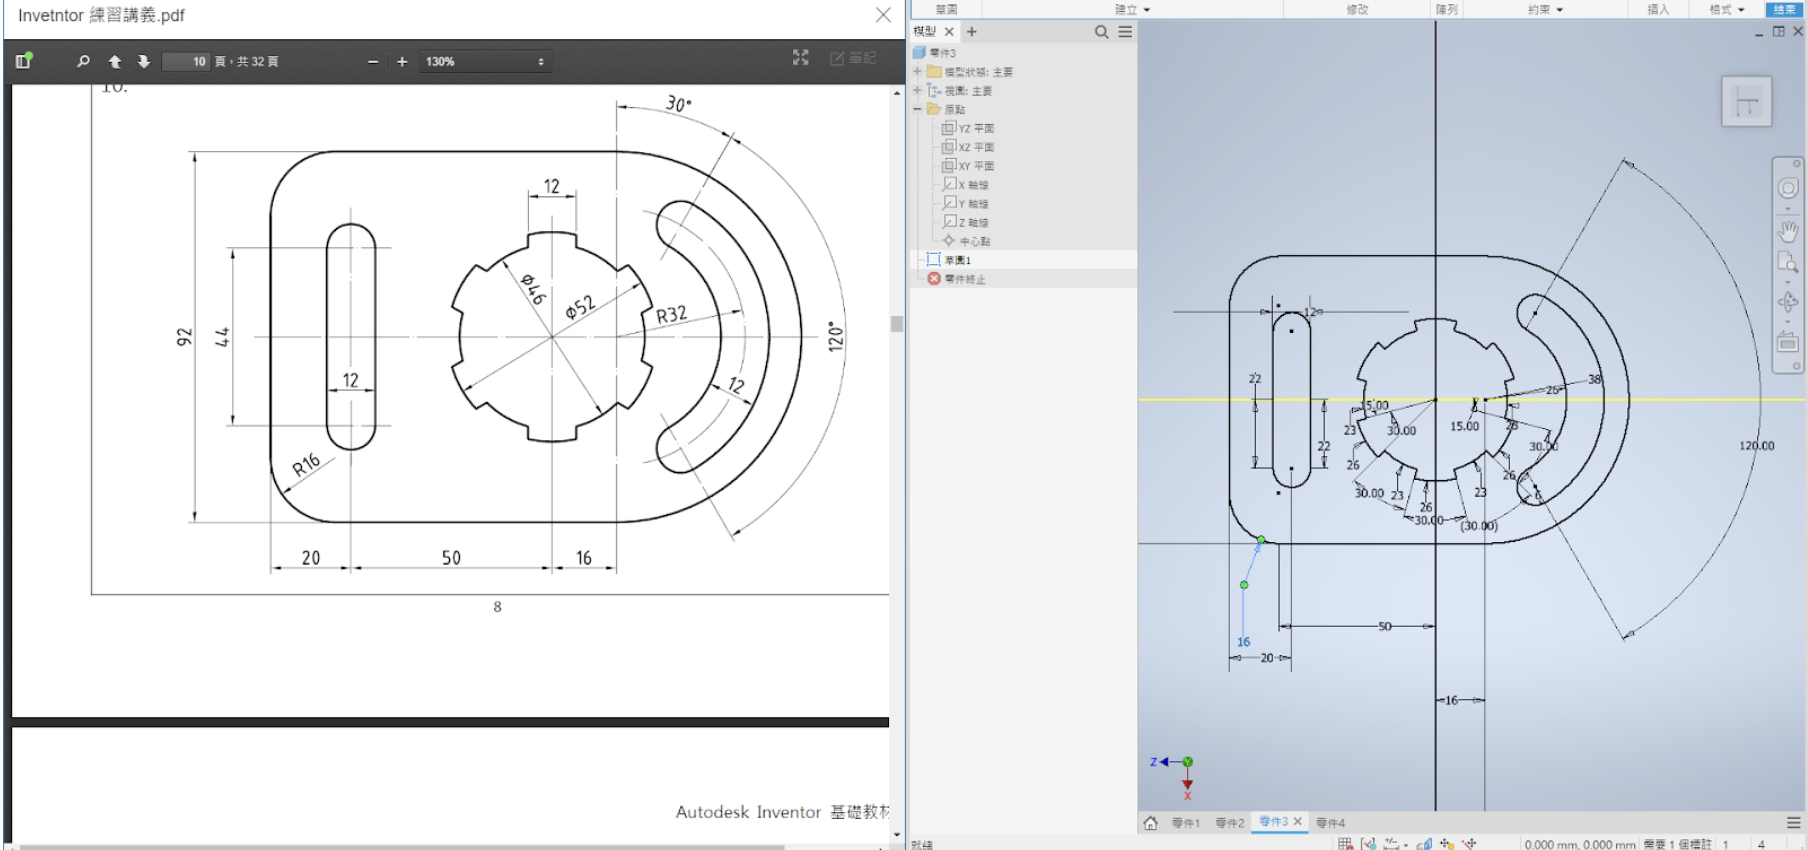
\includegraphics[width=0.7\textwidth]{./images/course_cad_draft1.png}
        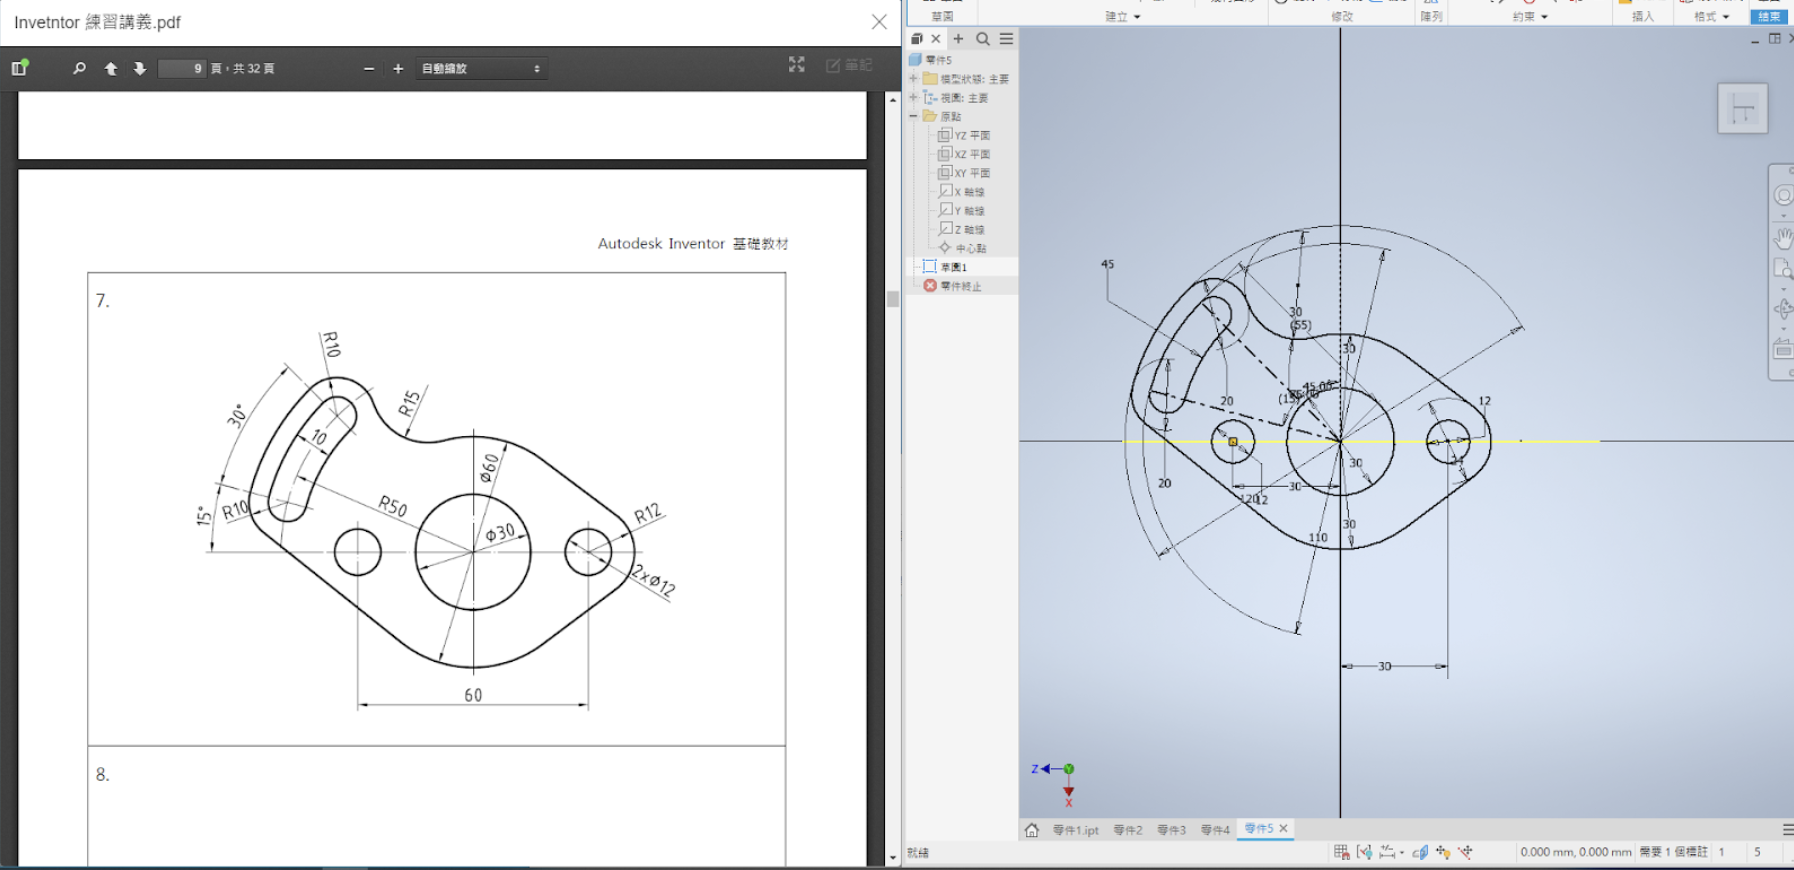
\includegraphics[width=0.7\textwidth]{./images/course_cad_draft2.png}
        \caption{課堂中所繪製的草圖}
        \label{fig:course_draft}
    \end{figure}
    \begin{figure}[h]
        \centering
        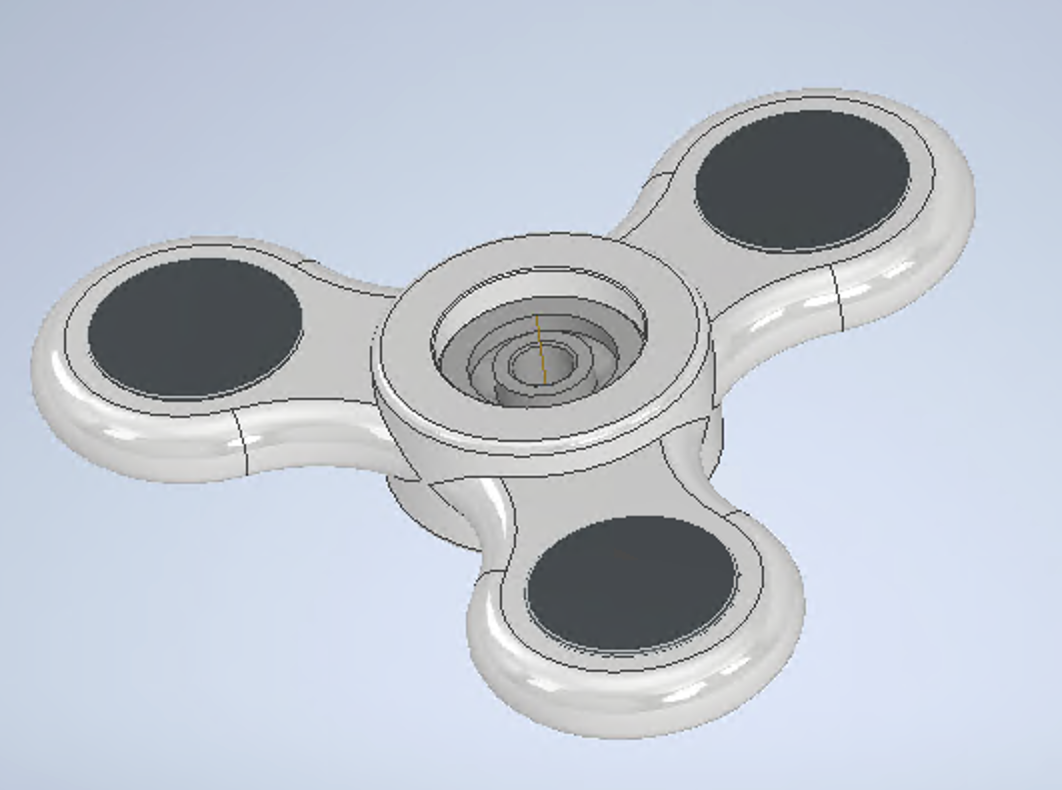
\includegraphics[width=0.4\textwidth]{./images/fidget_spinnner.png}
        \caption{指尖陀螺模型}
        \label{fig:figet_spinnner}
    \end{figure}

    \newpage

    \section{基礎電學}

    在這個部分老師除了告訴我們之後製作無刷馬達所需知識外,也向我們科普了許多相關知識,例如N型與P型半導體的差異、電晶體原理、達靈頓電路、電動勢與反向電動勢等。而以下便一一列舉。

    \subsection{半導體}
    \begin{enumerate}
        \item N型半導體:在半導體材料中,摻雜了能提供自由電子的雜質,這些自由電子可以自由移動,因此N型半導體的導電性較純淨的半導體高,而其電子濃度亦較高。
        \item P型半導體:在半導體材料中,摻雜了能提供正電洞的雜質,這些正電洞可以自由移動,因此P型半導體的導電性較純淨的半導體高,而其電洞濃度亦較高。
    \end{enumerate}

    \subsection{電晶體與二極體}
    \begin{enumerate}
        \item 電晶體:電晶體是一種半導體元件,由三個半導體層組成,分別是基極、發射極和集極。當基極與發射極之間的電壓大於一定值時,電晶體便會開啟,並且能夠控制大電流。
        \item 二極體:二極體是一種半導體元件,由P型半導體和N型半導體組成,當二極體的極性與電壓方向一致時,電流能夠通過,反之則無法通過。
    \end{enumerate}

    \subsection{達靈頓電路}
    \begin{enumerate}
        \item 介紹:達靈頓電路是一種由兩個電晶體組成的放大電路,能夠將輸入的微弱電流放大成較大的電流。
        \item 原理:當輸入電流通過第一個電晶體時,會使得第一個電晶體開啟,並且將電流放大,進而使得第二個電晶體開啟,並且將電流再次放大,最後輸出的電流會是輸入電流的數倍,因此若手指觸碰到輸入端,人體的微弱電流便能夠使得達靈頓電路輸出較大的電流,進而點亮燈泡。
        \item 實作如Figure \ref{fig:darlington}
              \begin{figure}[h]
                  \centering
                  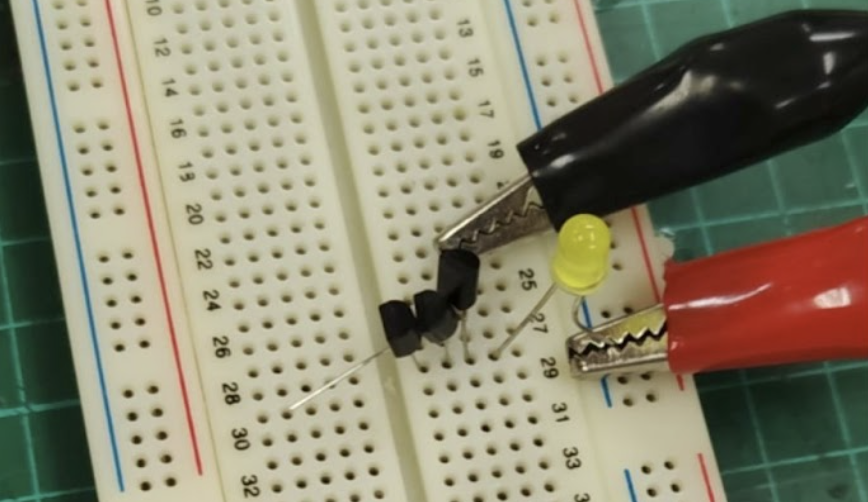
\includegraphics[width=0.45\textwidth]{./images/darlington_1.png}
                  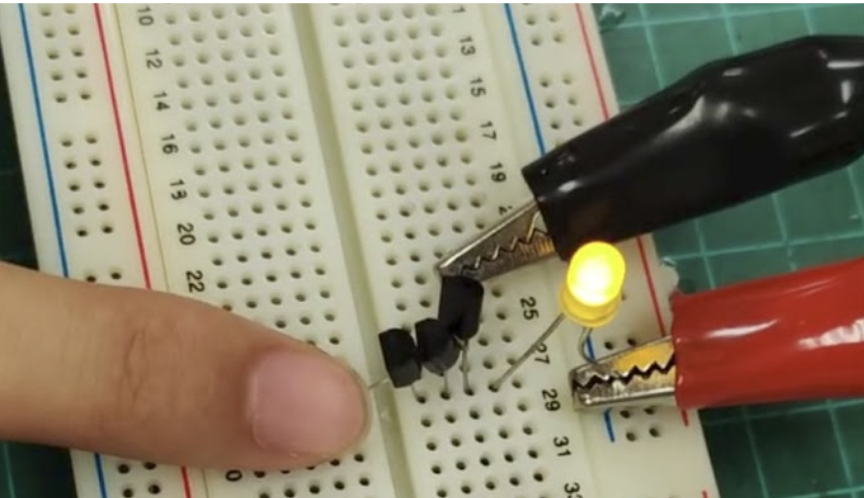
\includegraphics[width=0.45\textwidth]{./images/darlington_2.png}
                  \caption{達靈頓電路實作}
                  \label{fig:darlington}
              \end{figure}
    \end{enumerate}

    % TODO: 看這些東東
    % ! https://youtu.be/dwOe3r_wNDM?list=PLTQ2T0cDHYPcVTYiq7vixt4-AMp2wIFG5
    % ! https://youtu.be/mc979OhitAg?list=PLWv9VM947MKjuqlJVp5m_Edf66SrFSHx2
    % ! https://youtu.be/6Iqhx56RaXQ?list=PLTQ2T0cDHYPcVTYiq7vixt4-AMp2wIFG5
    % ! https://www.qsl.net/bv3fg/tech/BJTds.htm
    \subsection{電動勢與反向電動勢}

    \newpage

    \section{無刷馬達專題}

    \subsection{專案目標}
    \label{sec:goal}
    \begin{enumerate}
        \item 設計與製作轉速超過10000rpm效能的馬達(25W以內)
        \item 認識各參數對轉速的影響
        \item 認識電子元件的動作原理
        \item 熟練建模軟體協助專題製作
        \item 活用加工工具協助專題製作
        \item 設計測速工具協助觀察馬達運作
        \item 體驗專題製作歷程並編寫完整報告
    \end{enumerate}

    \subsection{分工}
    經過前段時期的建模與電路實習課程之後,老師讓我們自行依據個人專長,設定六個工作部門,期待我們集結不同屬性的人設,共同完成這一項工程專題活動。
    \begin{enumerate}
        \item PM(Project Manager):管理與支援工作,並匯整製作專題報告
        \item ME(Mechanical Engineer):科學探索與機械參數設計、主導構想
        \item QT(Quality Testing Engineer):科學探索與機械參數設計、優化設計
        \item EE(Electric \& Electronic Engineer):電機研究與電路配線
        \item ID(Industrial Designer):馬達(轉子、定子、感測、測速)設計與建模
        \item PE(Process Engineer) :各部件(底座、轉子、定子、支架)加工與組裝
    \end{enumerate}

    由於我們這組人數比較少,因此我有兼任多個部門,而我主要負責的是QT、EE、PE以及ID。以下是我們專案進度表。
    \noindent
    \begin{table}[H]
        \begin{center}
            \setlength{\tabcolsep}{1.25mm}{
                \begin{tabularx}{\textwidth}{|c|c|Y|c|c|c|c|c|c|c|c|}
                    \hline
                    主責 & 支援  & 主題工作    & 11/6 & 11/13 & 11/20 & 11/27 & 12/4 & 12/11 & 12/18 & 12/25 \\
                    \hline
                    PM & All & 專題分工討論  & V    &       &       &       &      &       &       &       \\
                    \hline
                    PM & All & 雲端資料分享  & V    &       &       &       &      &       &       &       \\
                    \hline
                    PM & All & 確認專題條件  & V    &       &       &       &      &       &       &       \\
                    \hline
                    PE & All & 確認可用資源  &      & V     &       &       &      &       &       &       \\
                    \hline
                    PM & All & 搜尋與整理資料 &      & V     &       &       &      &       &       &       \\
                    \hline
                    ME & All & 閱讀與分析資料 &      &       & V     &       &      &       &       &       \\
                    \hline
                    ME & EE  & 瞭解科學原理  &      &       & V     &       &      &       &       &       \\
                    \hline
                    ME & QT  & 分析馬達原理  &      &       & V     &       &      &       &       &       \\
                    \hline
                    ME & All & 提出設計方案  &      &       & V     &       &      &       &       &       \\
                    \hline
                    PE & PM  & 擬定BOM表  &      &       & V     &       &      &       &       &       \\
                    \hline
                    PM & All & 採購與取得零件 &      &       & V     &       &      &       &       &       \\
                    \hline
                    ID & ME  & 轉子、定子建模 &      &       &       & V     & V    &       &       &       \\
                    \hline
                    ID & PE  & 底座、支架建模 &      &       &       & V     & V    &       &       &       \\
                    \hline
                    PE & ID  & 線圈加工組裝  &      &       &       & V     & V    & V     &       &       \\
                    \hline
                    PE & ID  & 底座支架組裝  &      &       &       &       &      & V     & V     &       \\
                    \hline
                    EE & QT  & 電路實驗與繪圖 &      &       & V     &       &      &       &       &       \\
                    \hline
                    EE & PE  & 電路配線與測試 &      &       &       & V     &      &       &       &       \\
                    \hline
                    QT & All & 成品調校修正  &      &       &       &       &      &       & V     &       \\
                    \hline
                    PM & All & 完成專題與報告 & V    &       &       &       &      & V     & V     & V     \\
                    \hline
                \end{tabularx}}
            \caption{專案進度表}
            \vspace{-1.5cm}
        \end{center}
    \end{table}
    \subsection{資料搜集}
    \begin{enumerate}
        \item 電磁科學(ME)
              \subitem 為了瞭解那些參數對轉子的轉速有影響,我們決定引入高二物理學過的轉動公式,可以知道在功率固定的情形下,必須使轉動慣量減小,而藉由微調半徑與質量等參數,能夠有效使轉速提升。再者,磁力也是決定轉速的一大參數,由高三所學過的必歐-沙伐定律可以知道磁力與電流一次方正比且與半徑一次方反比。綜上所述,藉由參數的調整,能夠使馬達狀態最佳化。
        \item 馬達工程(QT):
              \begin{enumerate}
                  \item 有刷馬達與無刷馬達的差異:無刷馬達使用電子元件驅動,無需維護,並提供穩定轉速。有刷馬達則因碳刷與整流子接觸磨損需維護。無刷馬達優勢包括維護低、速度穩定、轉矩平穩、功率大。 \cite{whatBLDC}
                  \item 直流無刷馬達原理: 直流無刷馬達(BLDC)的原理主要涉及馬達的基礎構造與運轉原理。這類馬達通常由定子(Stator)和轉子(Rotor)組成,並在定子和轉子間留有一定的空氣間隙。BLDC不使用電刷進行電流換相,轉速由繞組線圈的電壓決定。這類馬達需要透過驅動電路將直流電轉換成三相電流來運作。此外,BLDC的驅動方式,包括使用橋式電路與功率開關進行三相的電流換相,並透過霍爾元件偵測馬達永磁轉子的角度。\cite{BLDCtheory1,BLDCtheory2}
              \end{enumerate}
        \item 電子元件(EE):
              \begin{enumerate}
                  \item 霍爾IC:一種能準確監測磁場變化的裝置,適合用於感測物件位置與移動。其核心是霍爾元件,能將磁場轉換為電壓,並透過處理電路如運算放大器來強化信號。這種感測器可以分為數位輸出的霍爾效應開關、鎖存IC,以及類比輸出的線性霍爾效應感測器,各自有不同的應用範圍。該技術廣泛應用於各種設備,如筆記型電腦、冰箱門,以及馬達位置監測等。\cite{whatHall}
                  \item MOSFET:一種四端子的高輸入阻抗半導體元件,包括漏極(D)、源極(S)、閘極(G)和基體(B)。它們有增強型和耗盡型兩大類型,並根據導體材料進一步分為N通道和P通道。MOSFET在電子電路中通常用作開關或放大器,並且具有不同的封裝類型,以適應不同的應用需求。 \cite{whatMosfet}
              \end{enumerate}
        \item 自製馬達範例(ID、EE):
              \begin{enumerate}
                  \item 指尖陀螺轉化為電動馬達的方法,涵蓋從基本到進階的設計,並運用元件如電磁鐵、霍爾感知器和光學感應器,同時也提供相關電路和測速方式 \cite{Fidget_Spinner_Motors}
                  \item 在前文電磁科學的相關資料搜集後,應該要讓磁鐵與電磁鐵在同一平面上才能使馬達轉得更快,因此我們參考了一些自製馬達的範例,並且在此基礎上進行改良 \cite{BLmoterVideo}
              \end{enumerate}
    \end{enumerate}
    \subsection{BOM表}
    \renewcommand{\arraystretch}{0.93}
    \begin{table}[H]
        \begin{center}
            \setlength{\tabcolsep}{1.25mm}{
                \begin{tabularx}{\textwidth}{|c|Y|c|c|c|}
                    \hline
                    品項       & 規格                       & 數量 & 單位 & 來源 \\
                    \hline
                    強力磁鐵     & 10mm x 10mm x 4mm厚       & 10 & 顆  & 老師 \\
                    \hline
                    滾珠軸承     & 3(內徑)x 10(外徑) x 4mm(厚)   & 2  & 顆  & 蝦皮 \\
                    \hline
                    漆包線      & SWG28\#,0.35mm(線徑)x m(長) & 1  & 捲  & 露天 \\
                    \hline
                    MOSFET   & P80NF10                  & 1  & 顆  & 露天 \\
                    \hline
                    霍爾IC     & A3144                    & 1  & 顆  & 露天 \\
                    \hline
                    二極體      & 1N4007                   & 2  & 顆  & 老師 \\
                    \hline
                    電阻       & 1MΩ                      & 1  & 顆  & 老師 \\
                    \hline
                    電阻       & 1kΩ                      & 1  & 顆  & 老師 \\
                    \hline
                    單芯線      & AWG 22\#                 & 1  & 捲  & 老師 \\
                    \hline
                    PCB洞洞板   & 6 x 28 孔                 & 1  & 片  & 露天 \\
                    \hline
                    木板       & 90 x 200 x 11mm          & 1  & 片  & 老師 \\
                    \hline
                    樺木合板     & 3/3.6mm/5.6mm厚           & 1  & 片  & 老師 \\
                    \hline
                    直流電源供應器1 & 學校提供                     & 1  & 台  & 老師 \\
                    \hline
                    直流電源供應器2 & 學校提供                     & 1  & 台  & 老師 \\
                    \hline
                    帶鋸機      & 學校提供                     & 1  & 台  & 老師 \\
                    \hline
                    雷切機      & 100W,900x600mm           & 1  & 台  & 老師 \\
                    \hline
                    鑽床       & 1/2HP                    & 1  & 台  & 老師 \\
                    \hline
                    手提電鑽     & 10.8V                    & 1  & 隻  & 老師 \\
                    \hline
                    金工虎鉗     & 學校提供                     & 2  & 隻  & 老師 \\
                    \hline
                    F型夾      & 學校提供                     & 1  & 隻  & 老師 \\
                    \hline
                    耐熱膠帶     & 10mm                     & 1  & 捲  & 老師 \\
                    \hline
                    熱縮套      & Ø5                       & 1  & 條  & 老師 \\
                    \hline
                    機械螺絲     & 圓頭,M3L55                 & 11 & 根  & 老師 \\
                    \hline
                    彈簧墊片     & 4mm                      & 1  & 片  & 老師 \\
                    \hline
                    六角螺帽     & M3                       & 11 & 顆  & 老師 \\
                    \hline
                    棉線       & 白色                       & 1  & 捲  & 老師 \\
                    \hline
                \end{tabularx}}
            \caption{BOM表}
        \end{center}
    \end{table}
    \renewcommand{\arraystretch}{1}
    \newpage
    \subsection{製作過程}
    \subsubsection{3D建模}
    \begin{enumerate}
        \item 零件圖
              \begin{figure}[h]
                  \centering
                  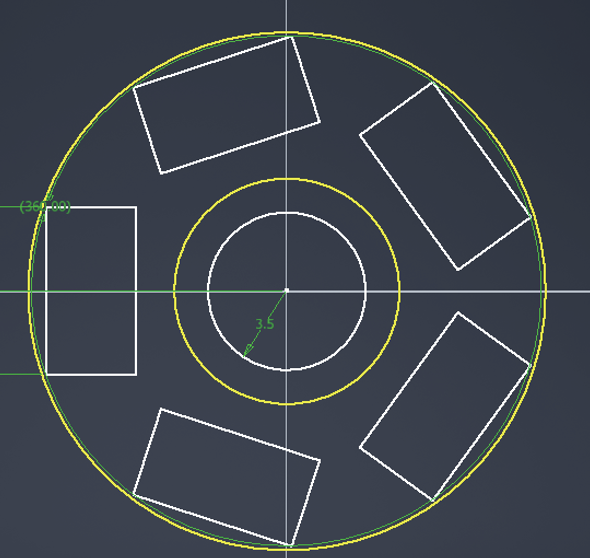
\includegraphics[height=0.2\textheight]{./images/cookie_draft.png}
                  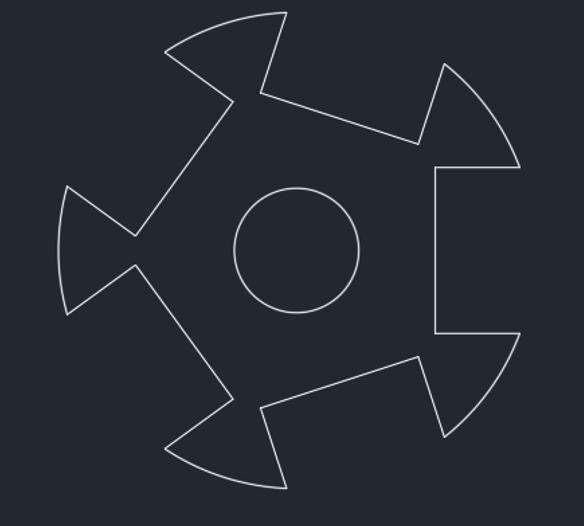
\includegraphics[height=0.2\textheight]{./images/filling_draft.png}
                  \caption{轉子架草圖}
              \end{figure}
              \begin{figure}[h]
                  \centering
                  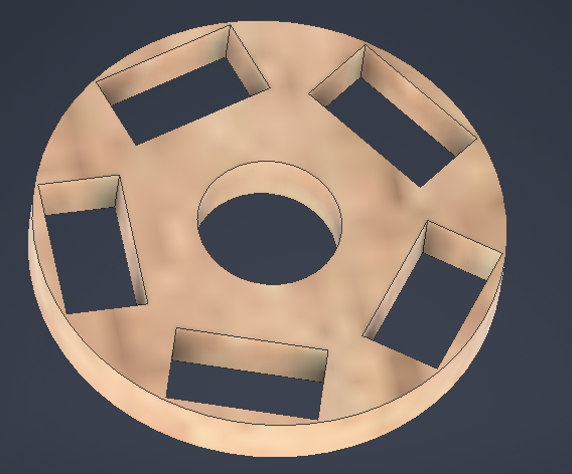
\includegraphics[height=0.2\textheight]{./images/cookie_3d.png}
                  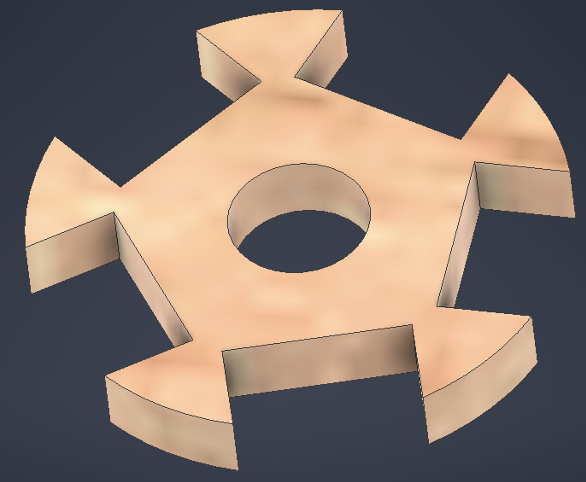
\includegraphics[height=0.2\textheight]{./images/filling_3d.png}
                  \caption{轉子架草圖(總共三層,上圖為上下兩層(cookie),下圖為中間層(filling))}
              \end{figure}
              \begin{figure}[H]
                  \centering
                  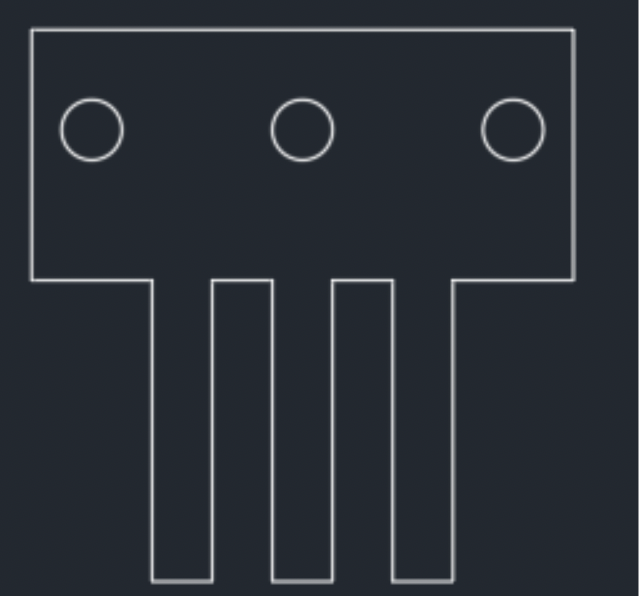
\includegraphics[height=0.2\textheight]{./images/stator_draft_1.png}
                  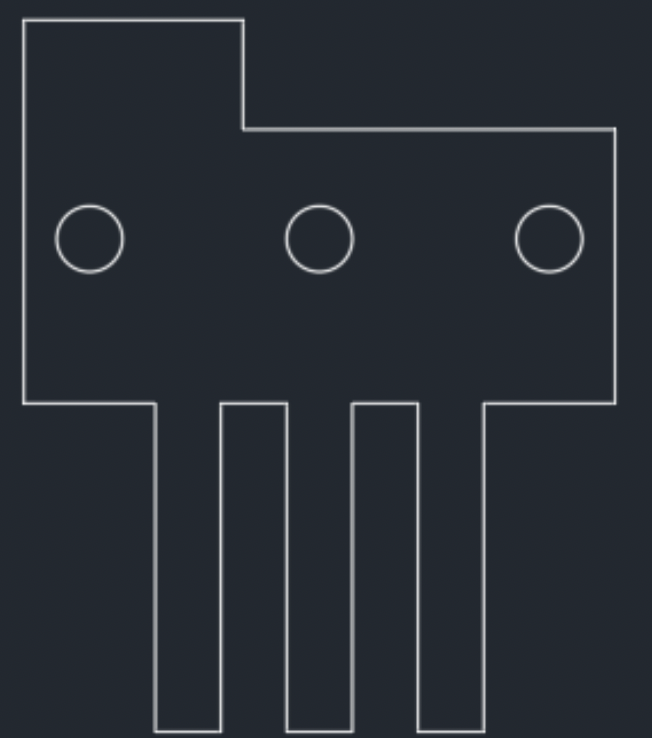
\includegraphics[height=0.2\textheight]{./images/stator_draft_2.png}
                  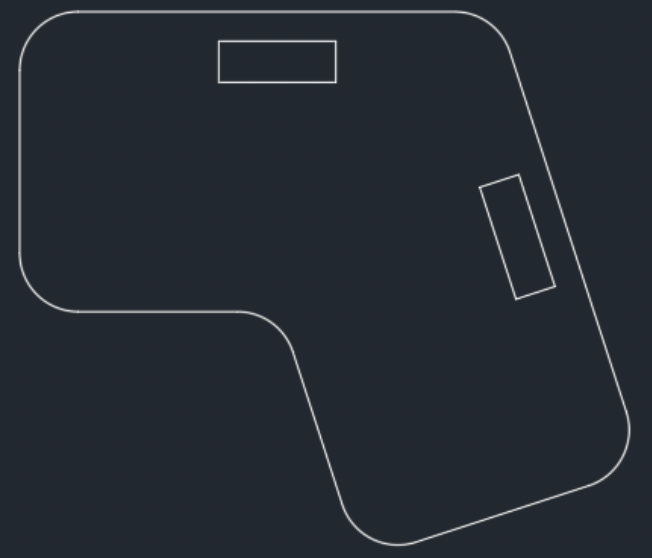
\includegraphics[height=0.2\textheight]{./images/hall_frame_draft.png}
                  \caption{定子架(前兩個)與霍爾感知架草圖(第二個定子架突出處是為接合霍爾感知架)}
              \end{figure}
              \newpage
        \item 組裝圖
              \begin{figure}[h]
                  \centering
                  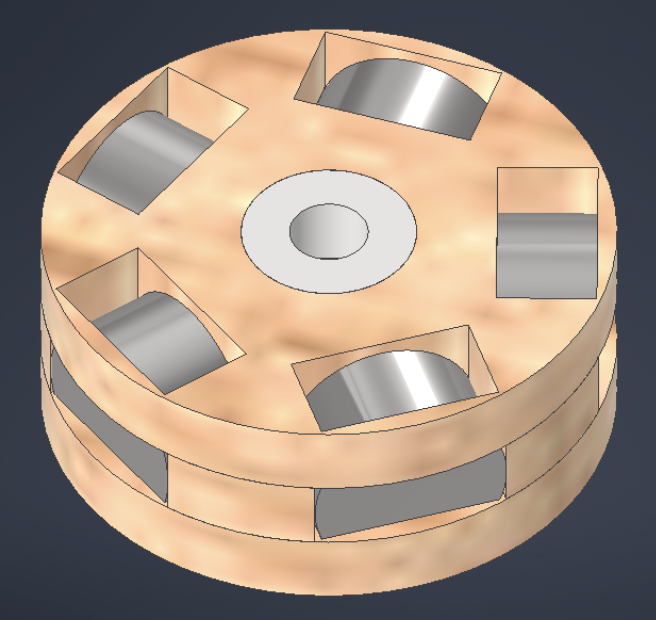
\includegraphics[height=0.18\textheight]{./images/rotor_3d.png}
                  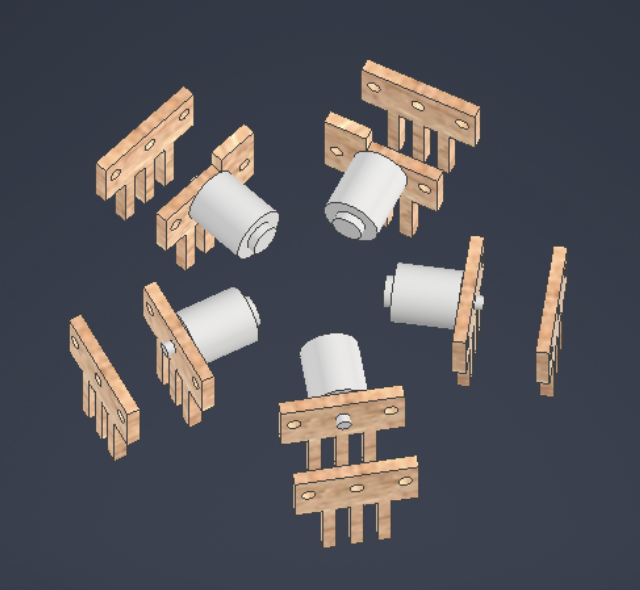
\includegraphics[height=0.18\textheight]{./images/stator_3d.png}
                  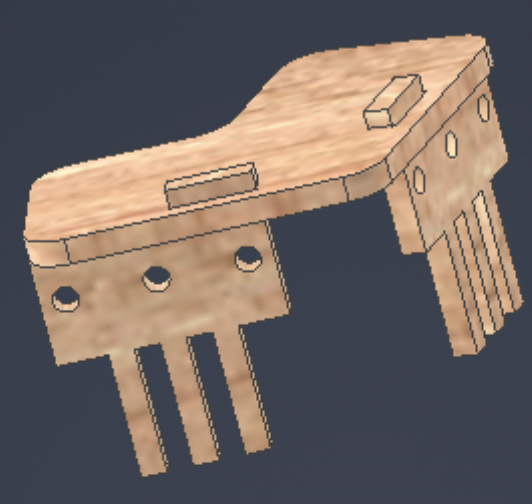
\includegraphics[height=0.18\textheight]{./images/hall_frame_3d.png}
                  \caption{轉子、定子、霍爾感知支架3D組裝圖}
              \end{figure}
              \begin{figure}[h]
                  \centering
                  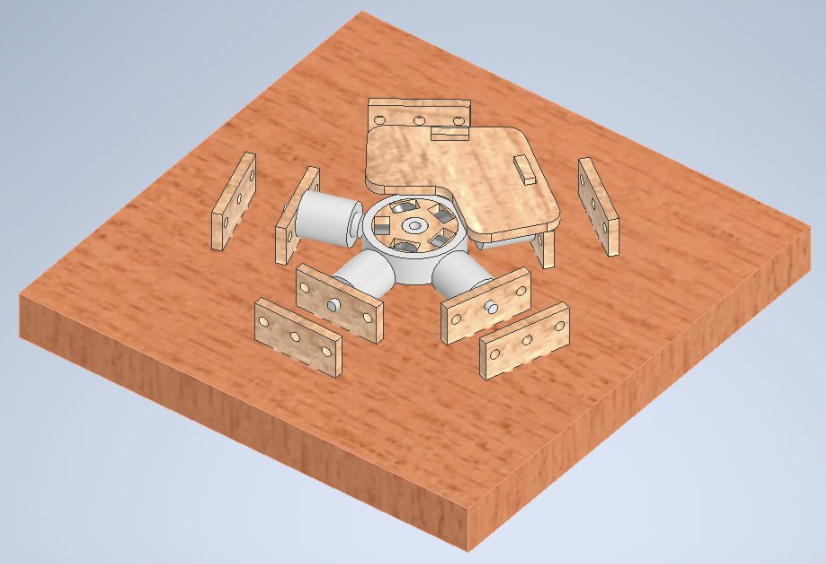
\includegraphics[width=0.5\textwidth]{./images/all_3d.png}
                  \caption{整組馬達模型3D組裝圖}
              \end{figure}
    \end{enumerate}

    \subsubsection{控制電路}
    \begin{enumerate}
        \item 手繪電路圖
              \begin{figure}[H]
                  \centering
                  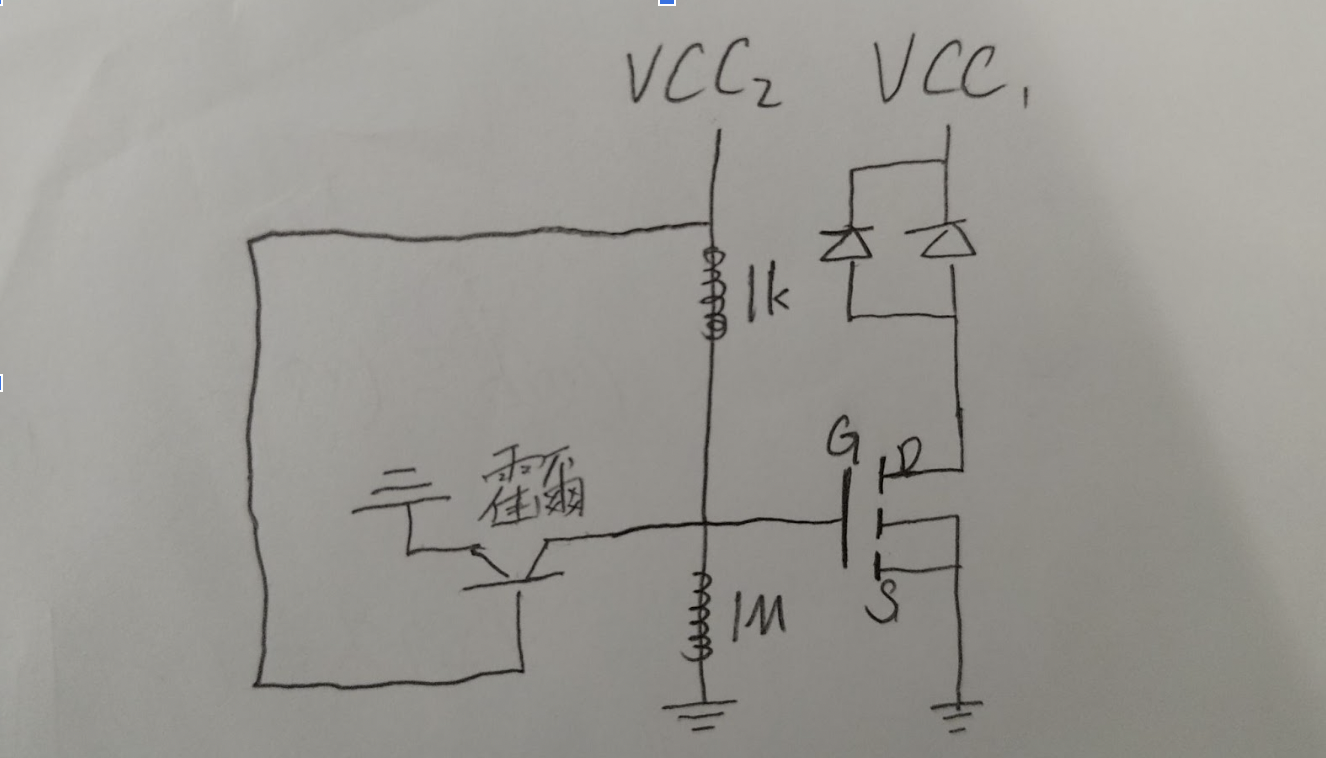
\includegraphics[width=0.7\textwidth]{./images/circuit_draft.png}
                  \caption{馬達控制電路手繪圖}
              \end{figure}
              \newpage
        \item Tinkercad 電繪電路圖與實體電路
              \begin{figure}[h]
                  \centering
                  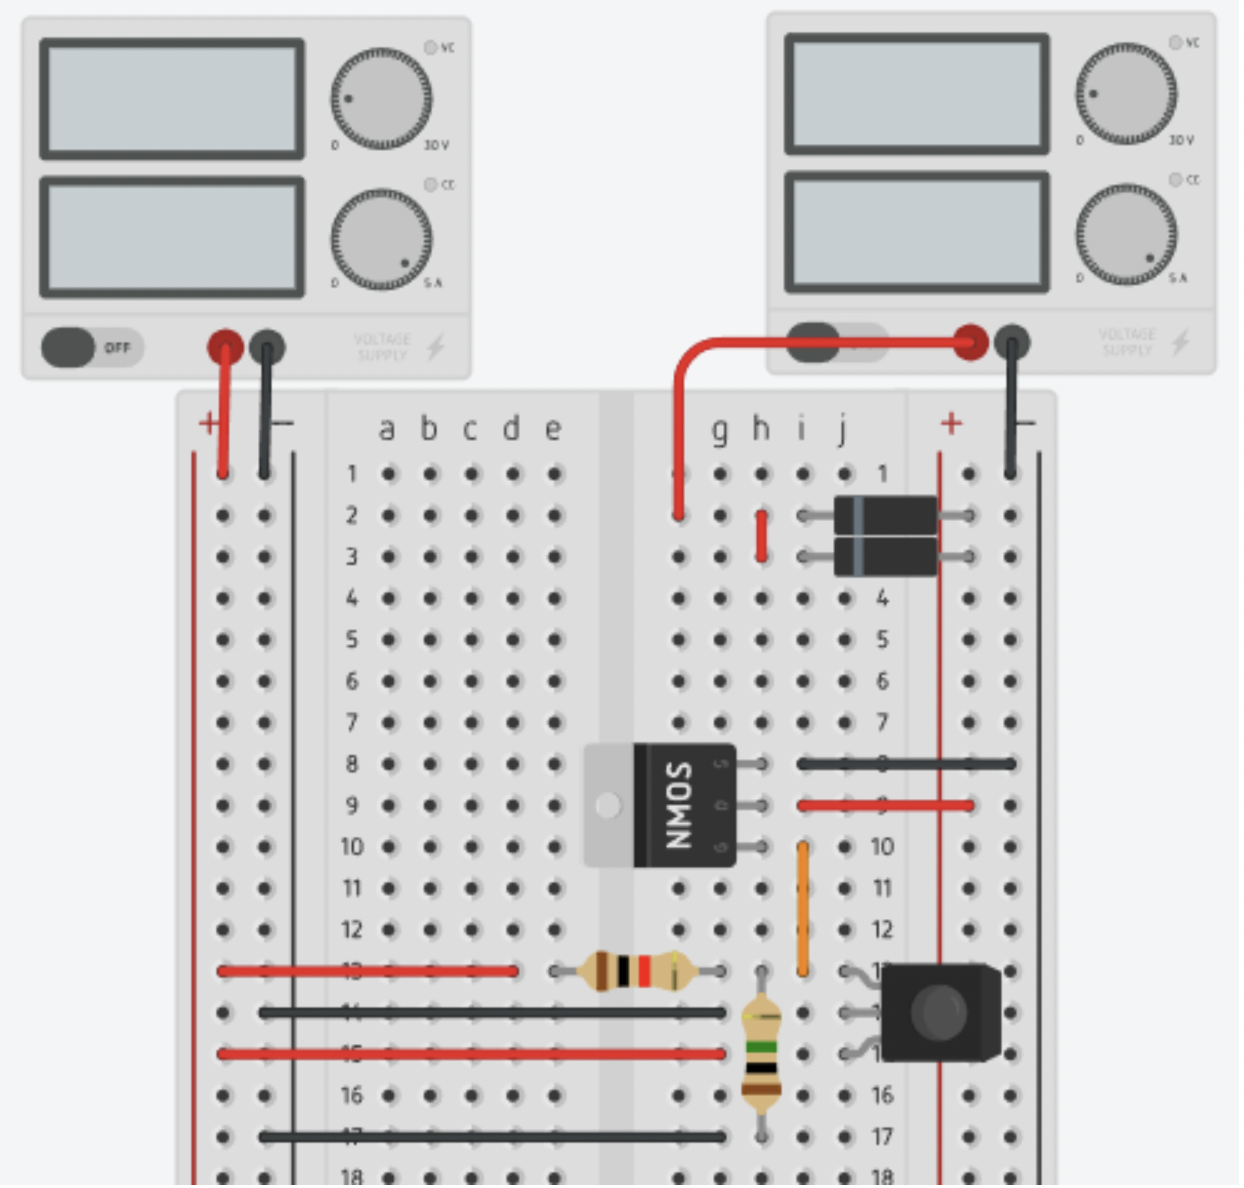
\includegraphics[height=0.25\textheight]{./images/circuit_digital.png}
                  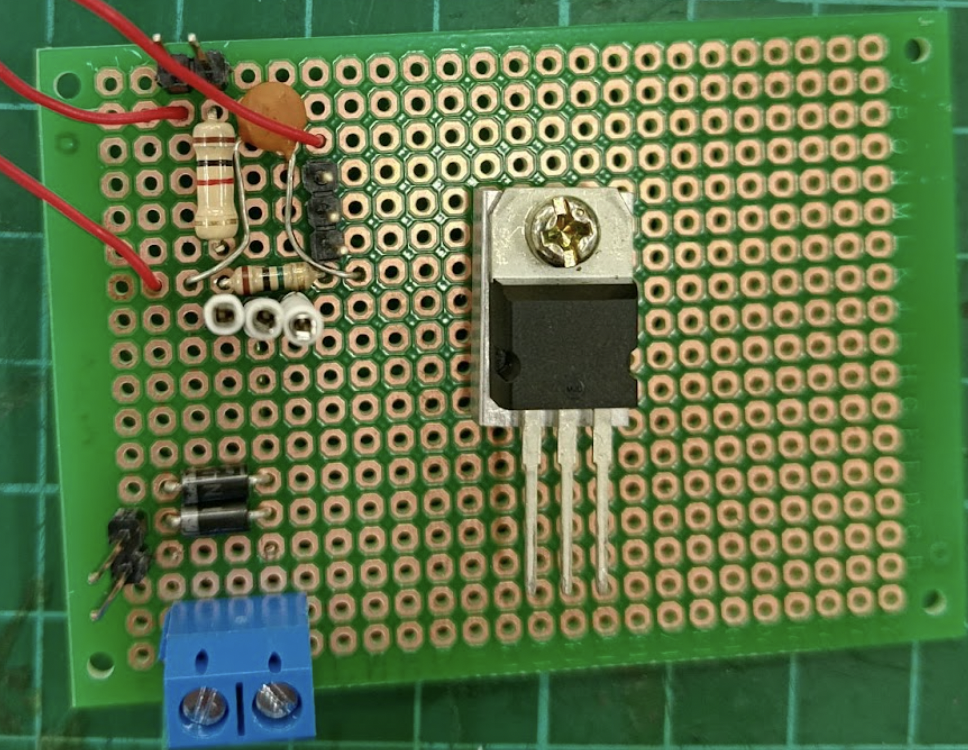
\includegraphics[height=0.25\textheight]{./images/circuit_real.png}
                  \caption{Tinkercad 電繪電路圖與實體電路}
              \end{figure}
    \end{enumerate}

    \subsection{調校分析}
    \begin{table}[H]
        \centering
        \begin{tabularx}{\textwidth}{|X|l|X|}
            \hline
            問題描述                                                                         & 轉速RPM & 擬修正說明                                                \\
            \hline
            從轉子側邊放置霍爾感知器,霍爾接近與遠離磁鐵時,電流有產生改變,但嘗試許久仍無法作動                                   & 0     & 可感測區域太小,試著將霍爾感知器移到轉子上方                               \\
            \hline
            成功轉動,但因仍是使用手持霍爾感知器因此無法穩定加速                                                   & 13000 & 先找到測試時能使轉子最快的大致位置,再利用膠帶將霍爾感知器固定在設計的固定架上,試圖不斷微調找到最佳位置 \\
            \hline
            轉速略趨穩定,但在加速過程中發現電流與電壓非恆定,似乎會隨轉速加速而不斷變化,因此很容易超過規定25W之規範,且發現在超過20W後轉速的變化就越來越小。 & 15000 & 可能能設計出自動的電壓調節器恆定瓦數,並利用視波器觀察反項電動式等會降低轉速之因素。           \\
            \hline
        \end{tabularx}
        \caption{測試過程}
    \end{table}

    \newpage
    \subsection{成果展示}
    各角度的照片與實測過程如Figure \ref{fig:demo},實測影片於\href{https://youtu.be/jbmlMec0Nww}{\textbf{此連結}}。重新回顧本專案目標(見\ref{sec:goal}),我們成功地設計與製作了一個在25W轉速高達15000rpm效能的馬達,並且在製作過程中,我們也學習到了各種電子元件的動作原理,熟練建模軟體,活用加工工具,並且編寫了完整報告,其中美中不足的是原先想利用Arduino進行轉速測量因時間不足而未能完成,只能改用手持測速器量測,但在人手不足的情況下,能夠達成如此成果,我們仍然感到非常滿意。

    \begin{figure}[h]
        \centering
        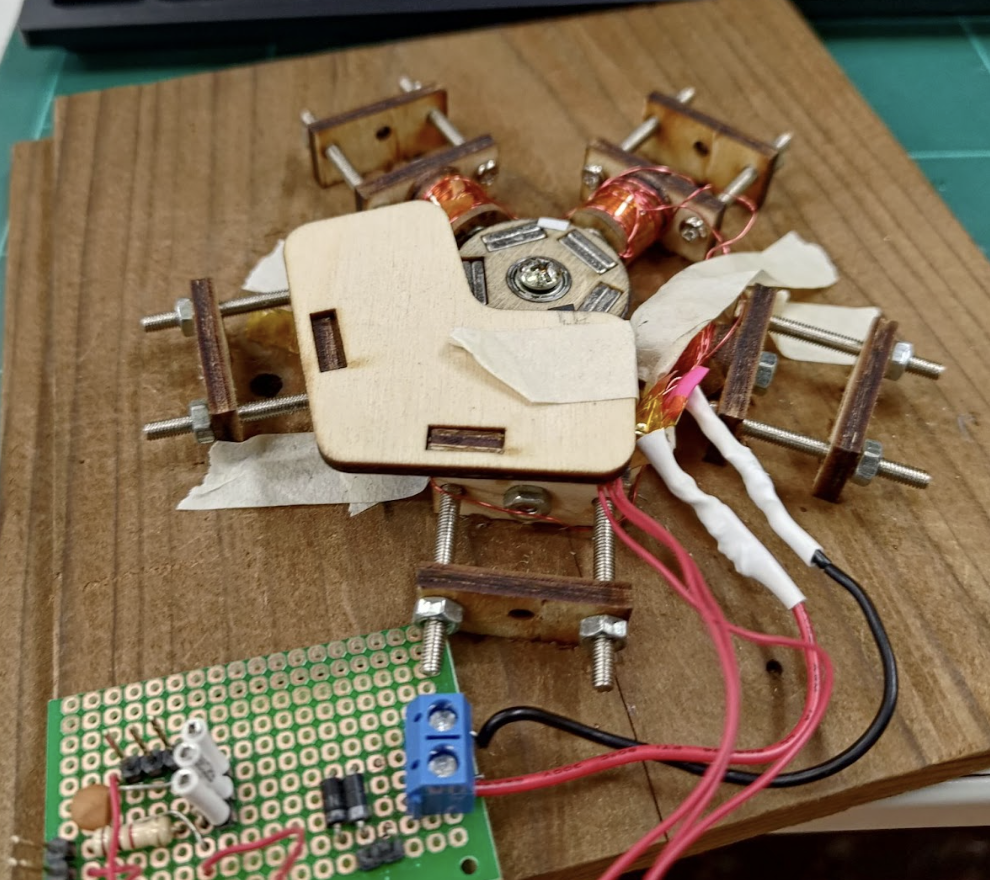
\includegraphics[height=0.2\textheight]{./images/finish1.png}
        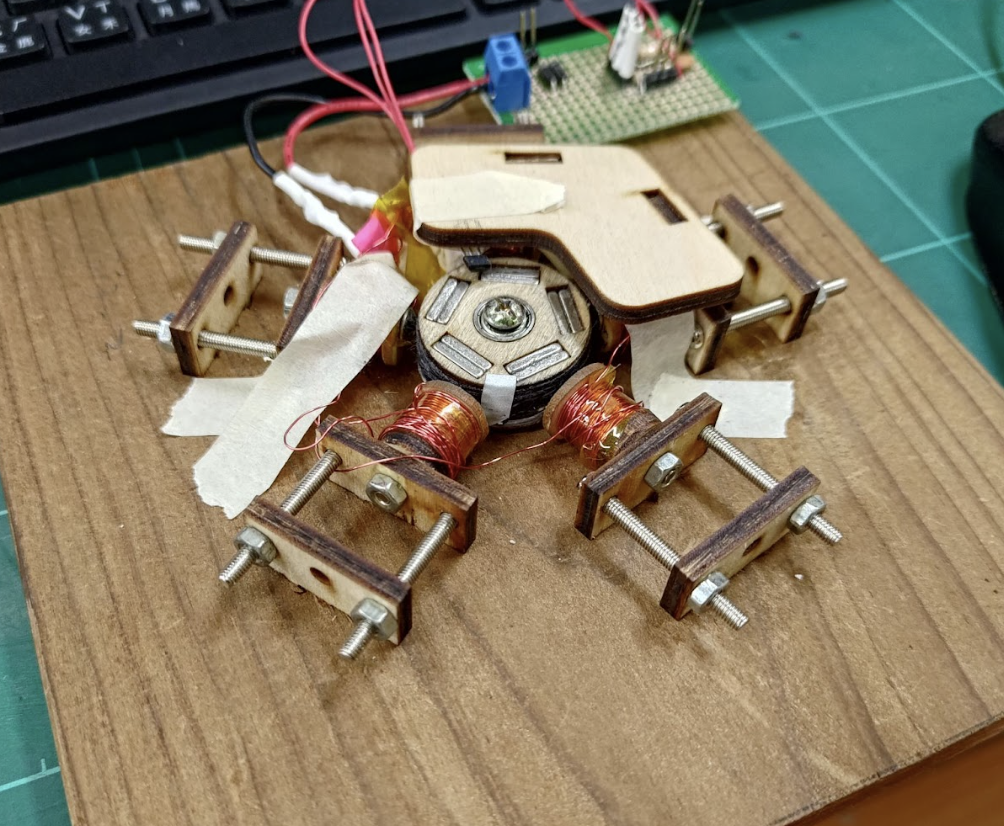
\includegraphics[height=0.2\textheight]{./images/finish2.png}
        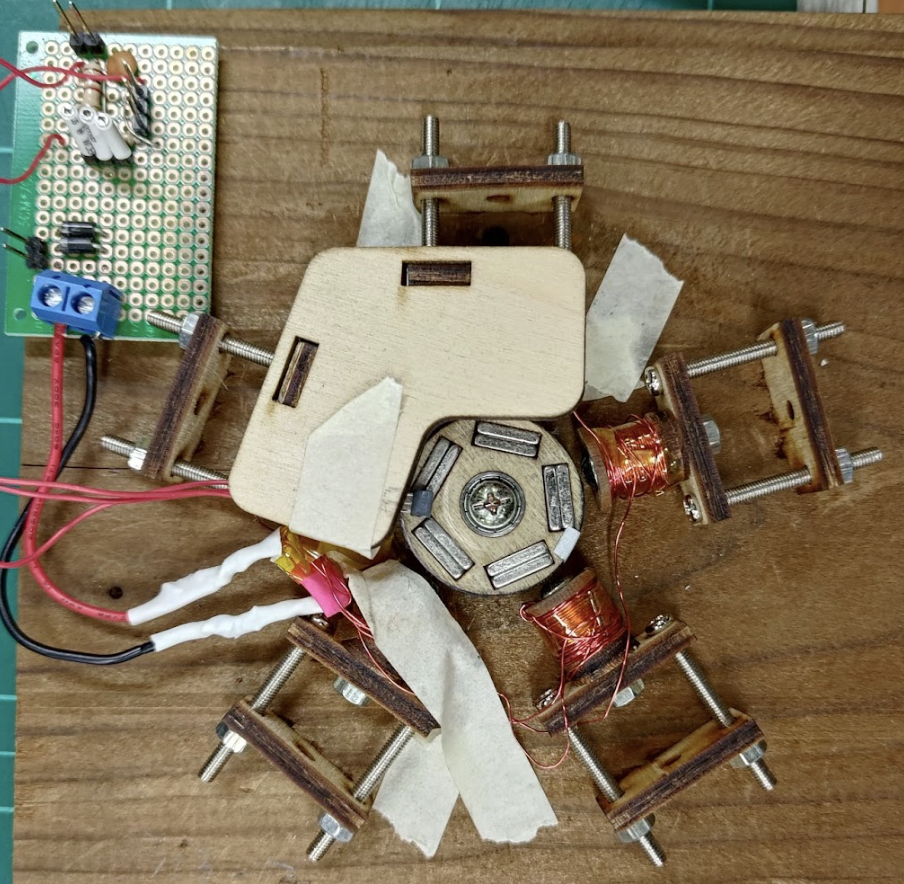
\includegraphics[height=0.2\textheight]{./images/finish3.png}
        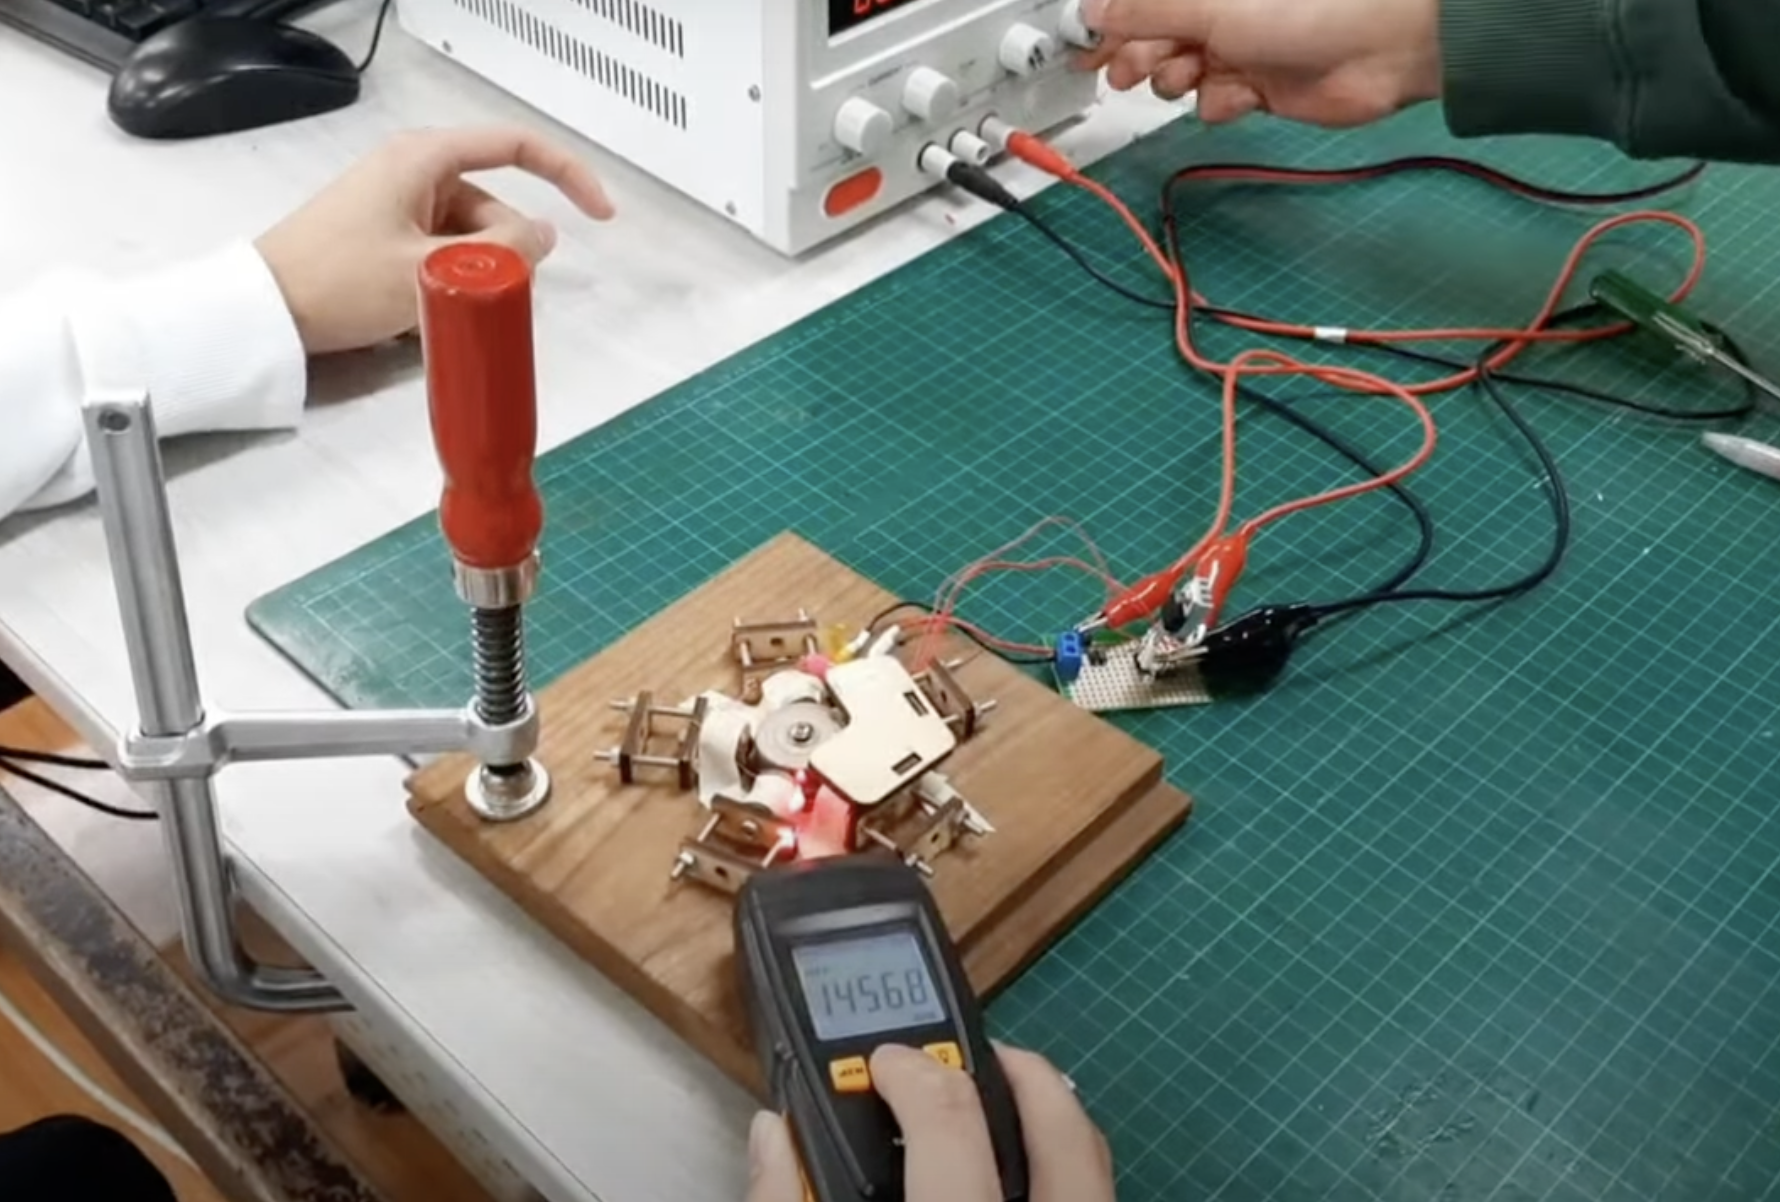
\includegraphics[height=0.2\textheight]{./images/demo.png}
        \caption{實體照片,實測影片於\href{https://youtu.be/jbmlMec0Nww}{\textbf{此連結}}}
        \label{fig:demo}
    \end{figure}
    \renewcommand{\arraystretch}{0.8}
    \begin{table}[H]
        \centering
        \begin{tabular}{|c|c|}
            \hline
            目標                            & 成果  \\
            \hline
            設計與製作轉速超過10000rpm效能的馬達(25W以內) & 完成  \\
            \hline
            認識各參數對轉速的影響                   & 完成  \\
            \hline
            認識電子元件的動作原理                   & 完成  \\
            \hline
            熟練建模軟體協助專題製作                  & 完成  \\
            \hline
            活用加工工具協助專題製作                  & 完成  \\
            \hline
            設計測速工具協助觀察馬達運作                & 未完成 \\
            \hline
            體驗專題製作歷程並編寫完整報告               & 完成  \\
            \hline
        \end{tabular}
        \caption{專案目標成果}
    \end{table}
    \renewcommand{\arraystretch}{1}
    \newpage
    \section{心得與反思}
    在課程中,我學習到一個無刷馬達是從無到有建構出來的,與以往製作專案不同,並非直接使用現成的套件拼湊,工程設計這堂課老師帶我們從半導體的原理,告訴我們何為N型、P型半導體,又是如何將排列組合作出二極體、電晶體,做出控制電流方向,甚至在達靈頓電路中更是直接感受到其能讓微弱電流增強的效果。在後續無刷馬達的電路中,運用先前所學,自己從頭做一塊電路板,通電,測試,最後馬達真的轉起來,這遠比Arduino拿一塊L298N控制馬達所帶來的成就感大多了。

    我很感謝在我探索電機的道路上有這段旅程,比起先前只是知道不同無刷馬達可能會因為不同廠牌的調校,在扭力、轉速上會有不同的表現,我更了解各種影響馬達的因素,氣隙、磁鐵、轉子、定子......各種要素互相影響,讓我能在未來挑選馬達時,有了更多切入的觀點,也在這段時間的學習中,讓我逐漸想在未來更深入了解電子、電路學的相關知識。

    此外,我因為考量到未來寫文章可能會頻繁使用\LaTeX,所以藉這次機會使用\LaTeX 撰寫本文(\href{https://github.com/moon-jam/engineering_design_learning_portfolio}{\bf{原始檔案}}),也在此過程中學習到許多排版技巧,相信對我未來的學術研究有很大的幫助。

    \newpage
    \nocite{*}
    \bibliographystyle{unsrt}
    \addcontentsline{toc}{section}{References}
    \bibliography{references}

\end{CJK*}
\end{document}